\chapter{Sintesi dell'Acido Acetico}

\section{Caratteristiche chimico-fisiche}
Temperatura di fusione = 16.6�C (289.7K)\\
Temperatura di normal ebollizione = 118.1�C (391.2K)\\
Solubile in acqua\\
Irritante\\
Limite di esplosivit� inferiore (in aria) = 5.4\% (v\/v) \\
Limite di esplosivit� superiore (in aria) = 16.0\% (v\/v)

\section{Principali impieghi}
L'acido acetico � il pi� importante tra gli acidi organici ed � noto fin dall'antichit�, infatti esistono documenti che confermano che era gi� in uso presso il popolo egizio.
La produzione annua dell \textit{Acido Acetico} � visibile in \tablename~\ref{tab:AcAc:ProduzioneAnnua}.
\begin{table}[htbp]
	\centering
		\begin{tabular}{p{1.8cm}p{1.8cm}p{1.8cm}p{1.8cm}p{1.8cm}p{1.8cm}}
			Anno	& USA		&	Europa 	& Giappone 	\\ \hline
			1990	& 1.71	&	1.26	 	&	0.46			\\
			1992	& 1.63	&	1.16		&	0.45			\\
			1995	& 2.12	&	1.47		&	0.57			\\\hline
		\end{tabular}
	\caption[Produzione annua di acido acetico tra il 1990 e il 1995.]{Produzione annua di acido acetico tra il 1990 e il 1995 ($\times 10^6$ tonn/anno).}
	\label{tab:AcAc:ProduzioneAnnua}
\end{table}

I principali utilizzi sono elencati in \tablename~\ref{tab:AcAc:Utilizzo}, ma la maggior parte di essi non sono altro che intermedi verso la produzione di altre sostanze (soprattutto resine e vernici).
\begin{table}[htbp]
	\centering
		\begin{tabular}{lp{5cm}c}
			Sostanza									& Formula 						& Percentuale \\ \hline
			Vinil acetato 						& \ce{CH_3COOCHCH_2} 	& 45			\\
			Anidride acetica					&	\ce{(CH_3CO)_2O} 		& 25			\\
			Esteri (isopropilacetato)	& \ce{CH_2COOCH(CH_2)_2} & 10 	\\
			Acetanilide	/ Acetammide	& \ce{Ph-NHCOCH_3} e \ce{CH_3CONH_2} & 9				\\
			Acido cloroacetico				& \ce{ClCH_2COOH}			& 2 \\
			Solvente 									& 			 	 						&	9 \\ \hline
		\end{tabular}
	\caption[Produzione annua di metanolo tra il 1978 e il 1995.]{Produzione annua di metanolo tra il 1978 e il 1995 ($\times 10^6$ tonn/anno).}
	\label{tab:AcAc:Utilizzo}
\end{table}

I principali processi noti per la produzione di acido acetico sono l'ossidazione dell'acetaldeide, la carbonilazione del metanolo, l'ossidazione di butani e altre vie (fermentativa). Nel mondo la produzione si � suddivisa come indicato in \tablename~\ref{tab:AcAc:MetodiProduzione}.
\begin{table}[htbp]
	\centering
		\begin{tabular}{lccc}
			Tecnica											& 1978	& 1989	& 1994	\\ \hline
			Ossidazione del acetaldeide	& 27 		& 27 		& 23		\\
			Carbonilazione del metanolo	&	47 		& 50 		& 58 		\\
			Ossidazione dei butani			& 7 		& 12		& 9			\\
			Altri												& 19 		& 11 		& 10		\\ \hline
		\end{tabular}
	\caption{Metodi di produzione nel mondo dell'acido acetico (percentuali).}
	\label{tab:AcAc:MetodiProduzione}
\end{table}

\section{Processo BASF}
Il processo BASF venne sviluppato nel 1960 in Germania e si basa sulla carbonilazione del metanolo tramite CO per ottenere acido acetico. Il processo avviene utilizzando un catalizzatore di cobalto ($CoI_2$) che viene attivato come spiegato di seguito.

Le condizioni in cui opera il processo sono di 220 - 250�C e 300 - 700Bar con una concentrazione di ioduro di cobalto di circa \textit{0.1M} .

La selettivit� raggiunta da questo processo � del 90\% rispetto al CO e al metanolo consumati, una resa in acido del 90\% rispetto al metanolo alimentato e del 70\% rispetto alla CO.

Da notare che la presenza di un ambiente acido (vedi le reazioni seguenti) costringe all'utilizzo, per il reattore, di leghe di ferro antiacido, aumentando i costi iniziali dell'impianto.

\subsection{Attivazione del catalizzatore}
Il vero catalizzatore della reazione � l'idro cobalto tetracarbonile, quindi in una fase iniziale vi deve essere l'attivazione del $CoI_2$ secondo la reazione riportata:
\begin{equation}
	2 CoI_2 + 2 H_2O + 10 CO \rightleftharpoons Co_2(CO)_8 + 4 HI + 2CO_2
	\label{rxn:AcAc:AttivazionCatCoI}
\end{equation}
in cui il cobalto passa dallo stato di ossidazione +2 a cobalto metallico. Successivamente il cobalto ottacarbonile diventa il vero promotore della reazione di carbonilazione del metanolo reagendo  con $CO$ e acqua:
\begin{equation}
	Co_2(CO)_8 + H_2O + CO \rightleftharpoons 2 HCo_2(CO)_4 + CO_2
	\label{rxn:AcAc:AttivazionCatCoI2}
\end{equation}

\subsection{Reazione principale}
Una volta che il catalizzatore � stato attivato la reazione procede formando dello ioduro di metile, consumando l'acido iodidrico prodotto precedentemente nella reazione \ref{rxn:AcAc:AttivazionCatCoI}:
\begin{equation}
	CH_3OH + HI\rightleftharpoons CH_3I + H_2O
	\label{rxn:AcAc:CH3I}
\end{equation}
Lo ioduro di metile formatosi reagisce con il catalizzatore tramite attacco nucleofilo tornando a liberare $HI$. Questo � lo stadio lento della reazione e controlla l'intera velocit� del processo:
\begin{equation}
	HCo_2(CO)_4 + CH_3I \rightleftharpoons CH_3Co_2(CO)_4 + HI
	\label{rxn:AcAc:SostNucl}
\end{equation}
Il prodotto cos� ottenuto fa migrare uno dei gruppi carbonilici per formare l'intermedio di reazione:
\begin{equation}
	CH_3Co_2(CO)_4 \rightleftharpoons  CH_3COCo_2(CO)_3
	\label{rxn:AcAc:MigrazioneCO}
\end{equation}
e successivamente, avendo liberato un punto di attacco per carbonili, si forma:
\begin{equation}
	CH_3COCo_2(CO)_3 + CO \rightleftharpoons  CH_3COCo_2(CO)_4
	\label{rxn:AcAc:AddizioneCO}
\end{equation}
A questo punto si ha un'eliminazione riduttiva che riporta il catalizzatore allo stato iniziale:
\begin{equation}
	CH_3COCo_2(CO)_4 + HI \rightleftharpoons CH_3COI + HCo_2(CO)_4
	\label{rxn:AcAc:EliminazRidut}
\end{equation}
Che reagisce con l'acqua liberata durante il processo per formare il prodotto desiderato:
\begin{equation}
	CH_3COI + H_2O \rightleftharpoons CH_3COOH + HI
	\label{rxn:AcAc:FormazAcAcFinale}
\end{equation}
Complessivamente il processo non porta alla formazione di prodotti indesiderati.

\subsection{Reazioni secondarie}
Essendo presenti sia $CO$ che $H_2O$ si hanno le medesime reazioni secondarie che si hanno nel processo di sintesi del metanolo, in particolare la reazione di \textit{schift}~(\ref{rxn:MetOH:Schift}) e le formazioni di \textit{HA}~(\ref{rxn:MetOH:HA2}, \ref{rxn:MetOH:HA3}, \ref{rxn:MetOH:HA4}). I sottoprodotti risulteranno, quindi, essere $CO_2$, $H_2$ e $HA$, oltre agli \textit{acetati} e \textit{formiati} di metile.

\section{Processo MONSANTO}
Il processo Monsanto viene applicato a partire dal 1969 e attualmente il 70\% dell'acido acetico prodotto viene sintetizzato tramite questo processo., in cui si utilizza un catalizzatore a base di rodio le cui fasi che portano alla formazione del prodotto sono simili a quelle che si hanno nel catalizzatore a base di cobalto; tuttavia, essendo i complessi a base di rodio bi� stabili di quelli al cobalto, sono necessarie condizioni operative pi� blande, infatti si hanno temperature di 185�C, pressioni di 25 - 35 Atm e concentrazioni di rodio di $10^{-3}$M. Nonostante ci� si ha una selettivit� del prodotto desiderato del 99.7\%.

L'inconveniente di questo processo � dato dal costo notevole del catalizzatore, infatti si utilizza $RhCl_3 \cdot 3 H_2O$ che ha un costo di circa 30.000 USD per mole. Proprio per questo motivo si punta ad ottimizzare il riciclo del catalizzatore e a ridurne le perdite a valori minimi.

\subsection{Attivazione del catalizzatore}
Come per il catalizzatore a base di cobalto anche il catalizzatore basato sul rodio deve subire una  prima fase di attivazione, infatti la molecola che funziona da catalizzatore � il $\left[RhI_2(CO)_2\right]^-$, complesso organometallico sufficientemente stabile.

\subsection{Reazione principale}
Una volta che il catalizzatore ha raggiunto la sua forma attiva la reazione prosegue con un'addizione ossidativa con ioduro metilico (che si forma in una fase successiva del processo) come descritto dalla seguente reazione:
\begin{equation}
	\left[RhI_2(CO)_2\right]^- + CH_3I \rightleftharpoons  CH_3\left[RhI_3(CO)_2\right]^-
	\label{rxn:AcAc:AddizOx}
\end{equation}
Successivamente si ha una migrazione del metile aggiunto:
\begin{equation}
	 CH_3\left[RhI_3(CO)_2\right]^- \rightleftharpoons  \left[RhI_3(CO)_2CH_3\right]^-
	\label{rxn:AcAc:MigrazMet}
\end{equation}
e una successiva addizione di $CO$ con una coordinazione dei ligandi:
\begin{equation}
	 \left[RhI_3(CO)_2CH_3\right]^- + CO \rightleftharpoons  \left[RhI_3(CO)_3CH_3\right]^-
	\label{rxn:AcAc:AddizCO}
\end{equation}
Da cui, tramite una eliminazione riduttiva, si libera il catalizzatore iniziale:
\begin{equation}
	 \left[RhI_3(CO)_3CH_3\right]^- \rightleftharpoons CH_3COI + \left[RhI_2(CO)_2\right]^-
	\label{rxn:AcAc:ElimRidut}
\end{equation}
Il catalizzatore torna in ciclo, mentre dal altro prodotto si ottiene l'acido acetico:
\begin{equation}
	 CH_3COI + H_2O \rightleftharpoons  CH_3COOH + HI
	\label{rxn:AcAc:FormazAcAc}
\end{equation}

L'intero processo pu� essere schematizzato come visibile in \figurename~\ref{fig:AcAc:SchemaCatRh}
\begin{figure}[htbp]
	\centering
		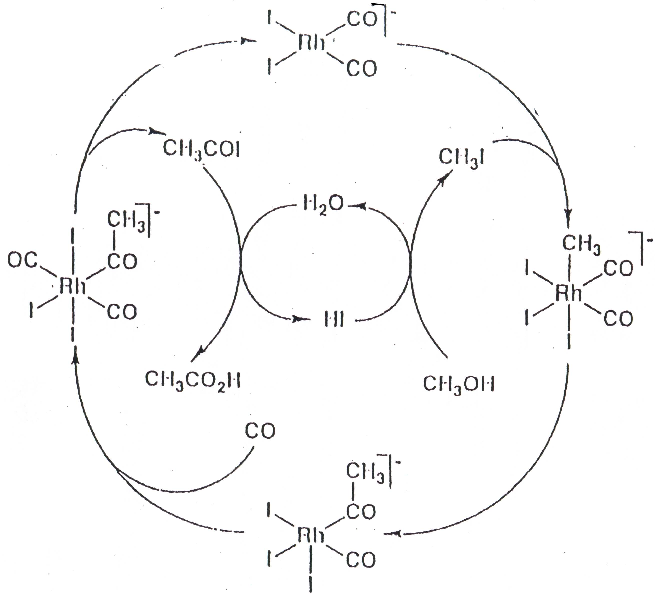
\includegraphics[width=0.70\textwidth]{image/ProcessoCatAcAcRh.pdf}
	\caption{Schema della reazione di formazione dell'acido acetico da $CO$ e $CH_3OH$ con catalizzatore a base di $Rh$}
	\label{fig:AcAc:SchemaCatRh}
\end{figure}

Essendo lo stadio lento dato dalla reazione l'addizione ossidativa dello ioduro di metile la velocit� di reazione complessiva pu� essere data da:
\begin{equation}
	 r = k \cdot [CH_3I] \cdot [Rh] \cdot [CH_3OK]^0 \cdot [CO]^0 \cdot [CH_3COOH]^0
	\label{rxn:AcAc:Cinetica}
\end{equation}
da cui � evidente che la velocit� di reazione dipende esclusivamente dalla concentrazione dello ioduro di metile e dalla concentrazione del catalizzatore di rodio, mentre non dipende dalla concentrazione del metanolo, del monossido di carbonio e dell'acido acetico.

\subsection{Reazioni secondarie}
Essendo presenti le seguenti specie: metanolo, acido acetico, monossido di carbonio e acqua sono presenti tutte le reazioni che portano alla formazione di sottoprodotti indesiderati, quali eteri (dimetil etere - $CH_3OCH_3$) ed esteri ($CH_3COOCH_3$). Possono anche esservi reazioni di \textit{metanazione}~(\ref{rxn:MetOH:Metanazione}) e di \textit{schift}~(\ref{rxn:MetOH:Schift}).

\section{Processo industriale}
Il processo industriale, indipendentemente dal catalizzatore utilizzato � composto da un \textit{reattore CSTR} in cui si ha la reazione per la formazione di acido acetico, seguito da un \textit{serbatoio di flash} da cui si separa il catalizzatore, che deve essere riciclato (vedi \ref{sec:AcAc:RecuperoCat}), dai composti volatili (metanolo, ioduro di metile e acido acetico) che devono essere separati. Questa operazione viene effettuata in una \textit{colonna di distillazione} dalla cui coda si ottiene acido acetico grezzo, mentre dalla testa si ricavano metanolo e ioduro di metile che viene riciclato. l'acido acetico grezzo viene, invece, inviato ad una serie di colonne di distillazione per la sua purificazione. Lo schema qu� descritto � visibile in \figurename~\ref{fig:AcAc:SchemaProcessoAcAc}.
\begin{figure}[htbp]
	\centering
		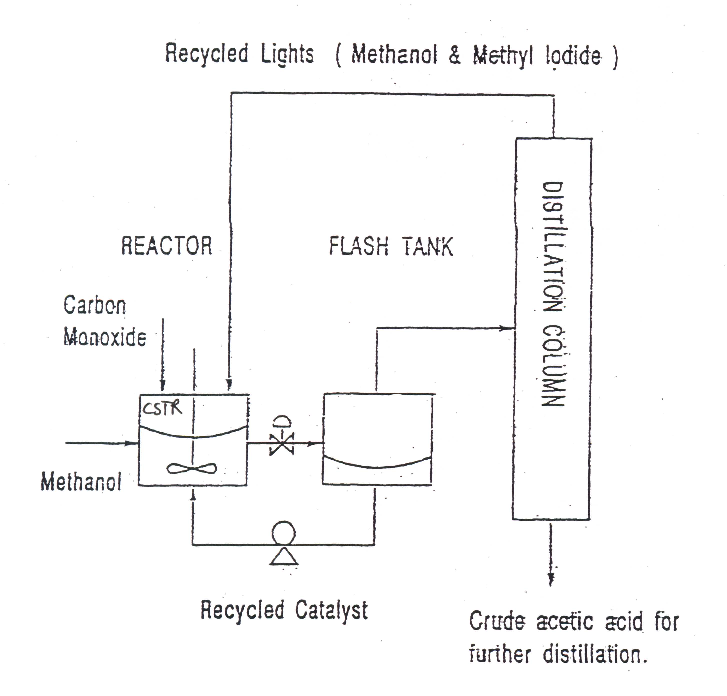
\includegraphics[width=0.70\textwidth]{image/SchemaProcessoAcAc.pdf}
	\caption{Schema di un generico impianto per la produzione di acido acetico a partire da metanolo e monossido di carbonio.}
	\label{fig:AcAc:SchemaProcessoAcAc}
\end{figure}

\subsection{Recupero del catalizzatore} \label{sec:AcAc:RecuperoCat}
Come accennato precedentemente il catalizzatore ha costi elevati, quindi � indispensabile il suo riciclo e soprattutto ridurre le perdite a valori minimi in modo da minimizzare i costi. Per fare questo la soluzione ottimale sarebbe l'utilizzo di un catalizzatore immobilizzato, in modo da avere un fase eterogenea e poter effettuare agevolmente la separazione. Tutt'oggi, per�, non si � riusciti a trovare un supporto che non porti a perdite rilevanti di Rh e di conseguenza si continua a ricorrere all'utilizzo di un catalizzatore disperso (fase omogenea) all'interno della massa di reazione e l'utilizzo di un flash per la sua separazione dai prodotti.

\subsection{Purificazione dell'acido acetico}
La purificazione dell'acido acetico avviene tramite l'utilizzo di colonne di distillazione. Dopo una prima separazione che permette di eliminare il metanolo e lo ioduro di metile si invia ad una serie di colonne di disidratazione, da cui si separa l'acqua e i prodotti pesanti dall'acido acetico, ottenendo come prodotto finale l'\textit{acido acetico glaciale} (99\%).

\section{Sviluppi futuri}
Dal 1997 � allo studio un catalizzatore di iridio che dovrebbe portare a una ulteriore riduzione delle pressioni di esercizio, nonch� all'aumento della velocit� di reazione e semplificazione del processo di separazione del catalizzatore dai prodotti all'uscita del reattore.